\apendice{Documentación técnica de Usuario }

\section{Requisitos previos}
\subsection{Modo usuario}
De forma previa a la utilización de la aplicación, se deberá tener instalado en el equipo lo siguiente: 
\begin{itemize}
\item \textbf{Sistema operativo}
\begin{itemize}
\item Windows
\end{itemize} 
\item \textbf{Distribución}
\begin{itemize}
\item Anaconda en su última versión estable 5.6, con la versión de Python 3.6. Dicha descarga se puede realizar a través del siguiente enlace: \url{https://www.anaconda.com/download/}
\end{itemize}
\item \textbf{Librerías  y Paquetes auxiliares}
\begin{itemize}
\item Matplotlib en la versión 2.0 o superior. En caso de no disponer de dicha librería actualizada, se puede actualizar con el siguiente comando: ``conda update --all''.
\item flask con el comando ``pip install flask''
\item flask\_marshmallow con el comando ``pip install flask\_marshmallow''
\item flasgger con el comando ``pip install flasgger''
\item SQLAlchemy con el comando ``pip install SQLAlchemy'' y el comando ``pip install flask\_sqlalchemy''
\end{itemize}
\item \textbf{Proyecto}
\begin{itemize}
\item Descargar o clonar el proyecto TFG-Sistema\_de\_recomendacion\_Asignaturas\_Optativas a través del siguiente enlace: \url{https://github.com/ClaraPalacios/TFG-Sistema_de_recomendacion_Asignaturas_Optativas/issues}
\end{itemize}
\item \textbf{Otros}
\begin{itemize}
\item PyQt5
\item PyDev en su versión 3.0-3.5
\end{itemize}
\end{itemize}

\subsection{Modo administrador}
En el modo administrador, además, será necesario el acceso a la API de GoogleDrive, de forma que serán necesario: 
\begin{itemize}
\item \textbf{Sistema operativo}
\begin{itemize}
\item Windows
\end{itemize} 
\item \textbf{Distribución}
\begin{itemize}
\item Anaconda en su última versión estable 5.6, con la versión de Python 3.6. Dicha descarga se puede realizar a través del siguiente enlace: \url{https://www.anaconda.com/download/}
\end{itemize}
\item \textbf{Librerías y Paquetes auxiliares}
\begin{itemize}
\item Matplotlib en la versión 2.0 o superior.  En caso de no disponer de dicha librería actualizada, se puede actualizar con el siguiente comando: ``conda update --all''.
\item flask con el comando ``pip install flask''
\item flask\_marshmallow con el comando ``pip install flask\_marshmallow''
\item flasgger con el comando ``pip install flasgger''
\item SQLAlchemy con el comando ``pip install SQLAlchemy'' y el comando ``pip install flask\_sqlalchemy''
\end{itemize}
\item \textbf{Datos Auxiliares}
\begin{itemize}
\item Clave secreta importada en el fichero JSON. 
\end{itemize}
\item \textbf{Proyecto}
\begin{itemize}
\item Descargar o clonar el proyecto TFG-Sistema\_de\_recomendacion\_Asignaturas\_Optativas a través del siguiente enlace: \url{https://github.com/ClaraPalacios/TFG-Sistema_de_recomendacion_Asignaturas_Optativas/issues}
\end{itemize}
\item \textbf{Otros}
\begin{itemize}
\item PyQt5
\item PyDev en su versión 3.0-3.5
\end{itemize}
\end{itemize}

\section{Ejecución del proyecto}


\section{Utilización}
Tras la ejecución del proyecto, se abrirá una pestaña en la que el usuario debe introducir su correo y contraseña. 

\subsection{Inicio sesión}
Para iniciar sesión, el usuario debe introducir su correo y contraseña, y en caso de introducirlo de forma correcta, se abrirá la pestaña principal.\ref{fig:E.2.1.1} En caso contrario, permanecerá dicha pestaña con los campos vacíos de nuevo para reintroducir los datos, mostrando en una ventana emergente el error obtenido.  
\begin{figure}[h]
\centering
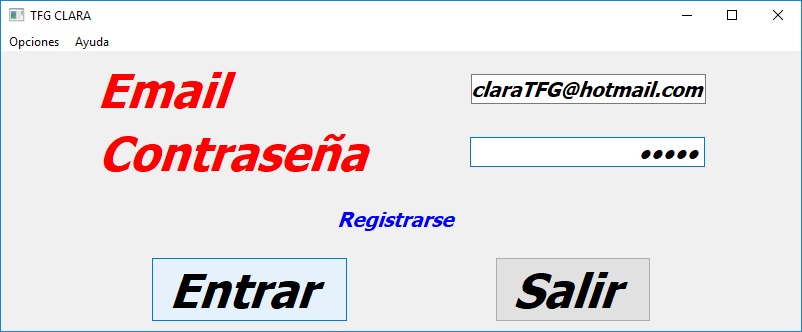
\includegraphics[width=0.80\textwidth]{INTERFAZ_Inicio_sesion_funcional}
\caption{Inicio de sesión}
\label{fig:E.2.1.1}
\end{figure}
\\En caso de haber obtenido un error introduciendo usuario o contraseña, aparecerá dicho mensaje: \ref{fig:E.2.1.2}
\begin{figure}[h]
\centering
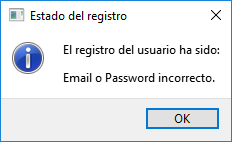
\includegraphics[width=0.80\textwidth]{Error_inicio_sesion}
\caption{Inicio de sesión}
\label{fig:E.2.1.2}
\end{figure}
\\Por otra parte, si es la primera vez que un usuario se registra por primera vez, debe pulsar el botón "Registrarse" como indica la siguiente figura \ref{fig:E.2.1.3}
\begin{figure}[h]
\centering
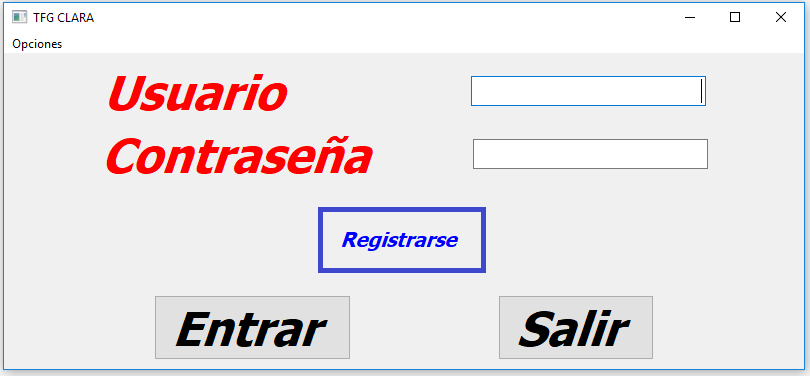
\includegraphics[width=0.80\textwidth]{para_registrarse}
\caption{Botón registrarse}
\label{fig:E.2.1.3}
\end{figure} 
\\Se abrirá una nueva pestaña en la que el usuario debe introducir su correo, su nombre y su contraseña:\ref{fig:E.2.1.4}
\begin{figure}[h]
\centering
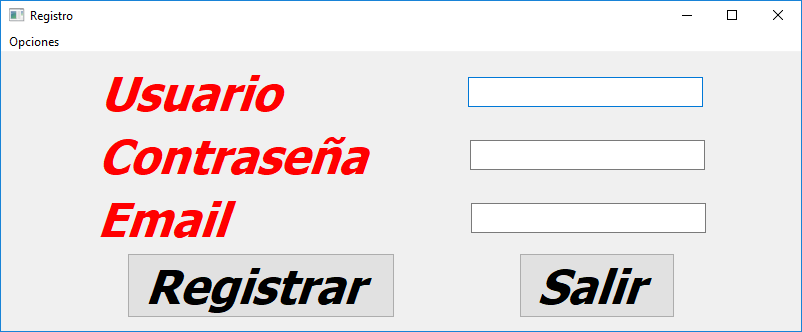
\includegraphics[width=0.80\textwidth]{Registrarse}
\caption{Pestaña de registro de usuario}
\label{fig:E.2.1.4}
\end{figure} 
\\De esta forma, si se ha registrado el usuario de forma correcta, volverá a aparecer la pantalla de inicio sesión para introducir el usuario y contraseña.
\subsection{Primera pestaña}
\subsubsection{Version1.0}
Tras iniciar sesión, aparecerá la siguiente pestaña: \ref{fig:E.2.1}
\begin{figure}[h]
\centering
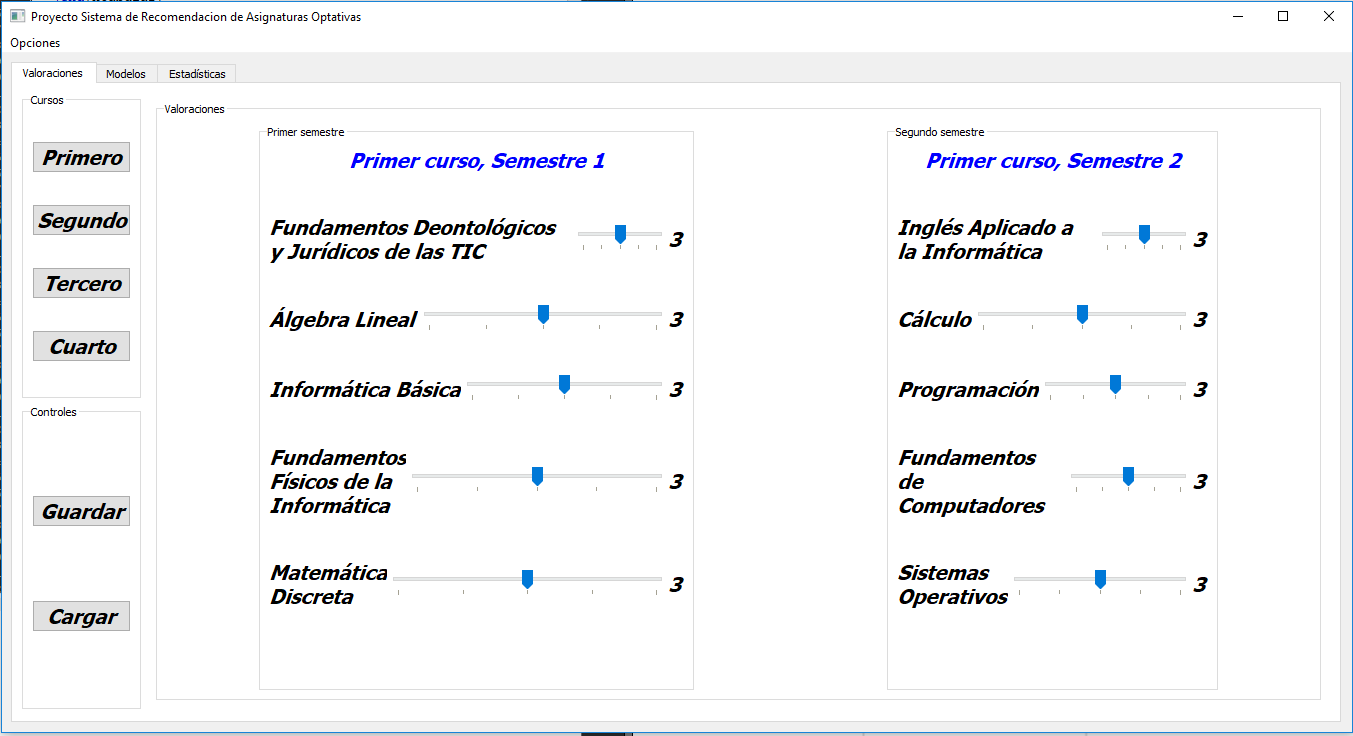
\includegraphics[width=0.80\textwidth]{INTERFAZ_Rellenado_Datos_V1-0}
\caption{Interfaz de rellenado de cuestionario}
\label{fig:E.2.1}
\end{figure}
Los cursos, son botones clicables, los cuales, al ser pulsados, muestran las asignaturas correspondientes a dicho año. \ref{fig:E.2.2}
\begin{figure}[h]
\centering
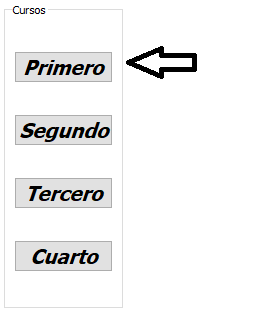
\includegraphics[width=0.80\textwidth]{cursos}
\caption{Cursos}
\label{fig:E.2.2}
\end{figure}

En caso de haberse registrado por primera vez, en el área central de la pantalla, las asignaturas constarán de valores medios, que deberán ser modificados por el usuario. \ref{fig:E.2.3}
\begin{figure}[h]
\centering
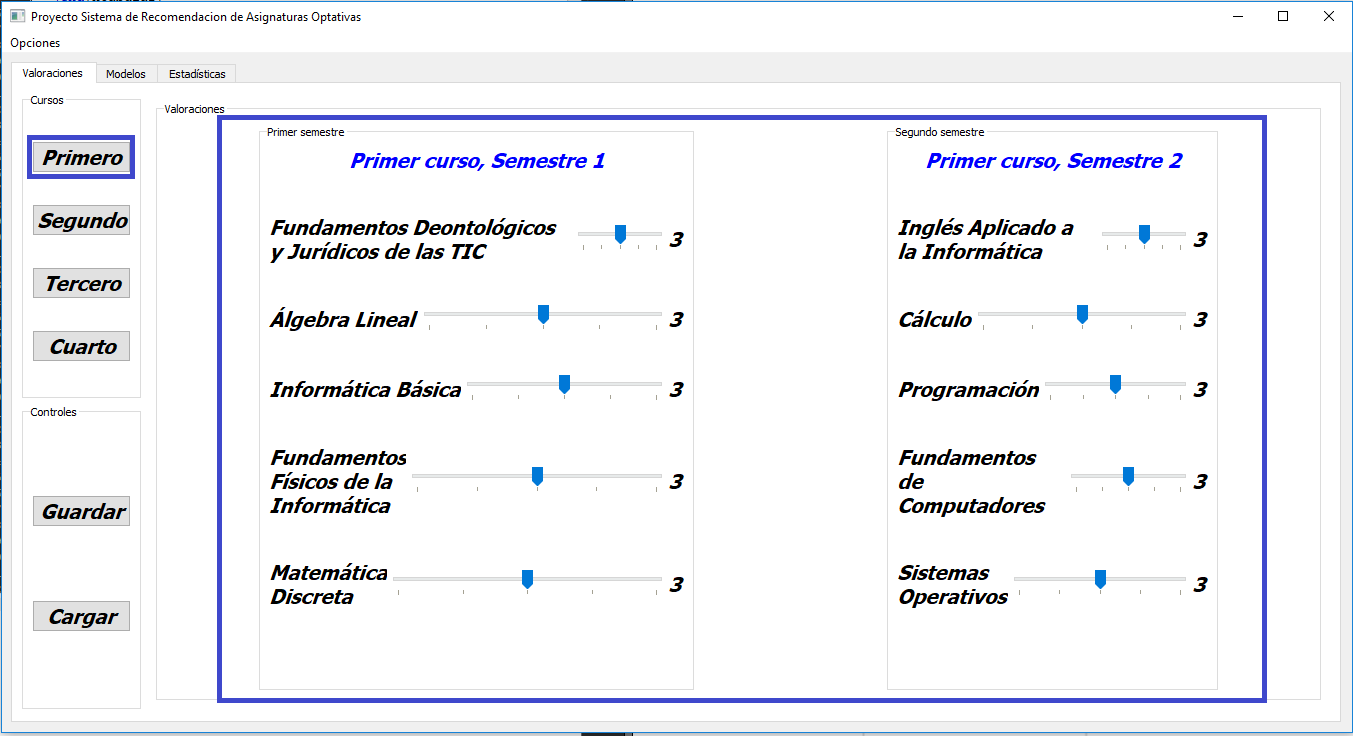
\includegraphics[width=0.80\textwidth]{INTERFAZ_Rellenado_Datos_Central_V1-0}
\caption{Parte central pestaña rellenado de datos}
\label{fig:E.2.3}
\end{figure}
Se pueden modificar las ponderaciones de las asignaturas bien con el ratón, arrastrando  slider, o bien con el teclado con las flechas izquierda y derecha. En la siguiente imagen se puede observar la diferencia entre utilizar el ratón y el teclado. \ref{fig:E.2.4}
\begin{figure}[h]
\centering
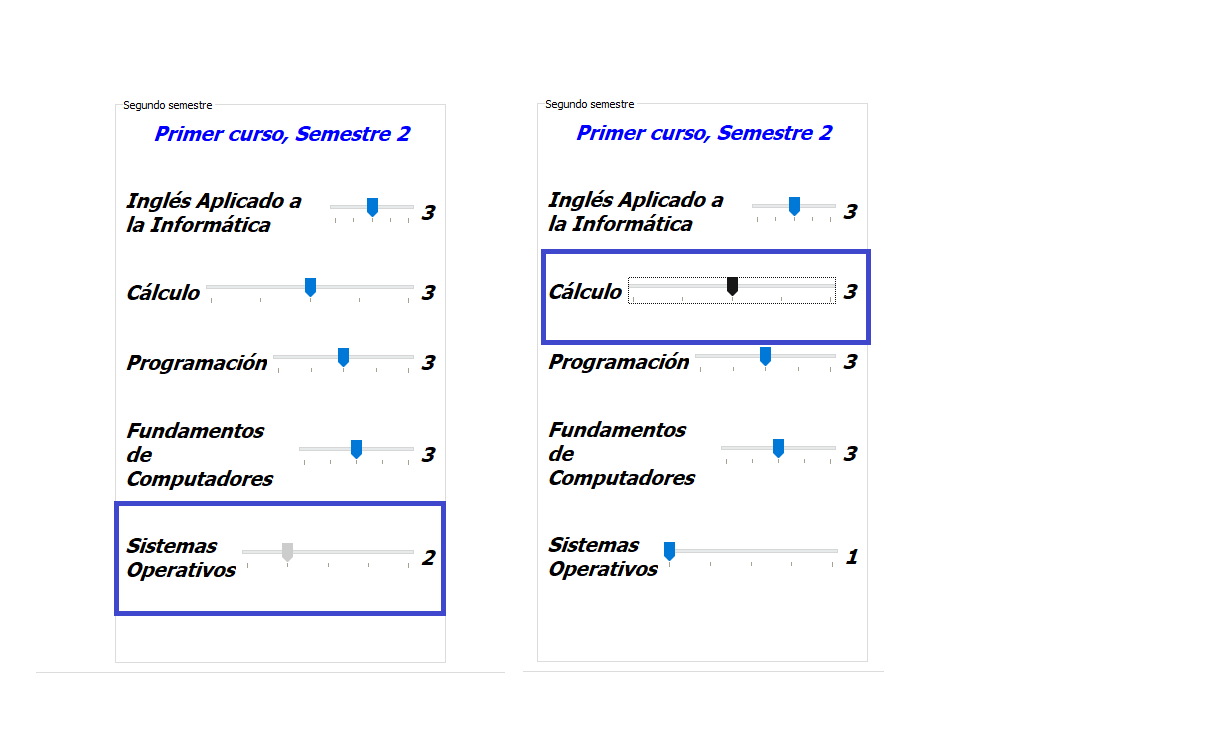
\includegraphics[width=0.80\textwidth]{INTERFAZ_Rellenado_Datos_Raton_V1-0}
\caption{Img Izq: Selección con ratón. Img Der: Selección con teclado}
\label{fig:E.2.4}
\end{figure}

En los botones de control, se permite \textbf{guardar} y \textbf{cargar} los datos. Al pulsar el botón guardar, se guardarán los datos introducidos de los cursos en un fichero binario, mientras que si se pulsa cargar, dichos datos se cargarán de forma automática. \ref{fig:E.2.5}
\begin{figure}[h]
\centering
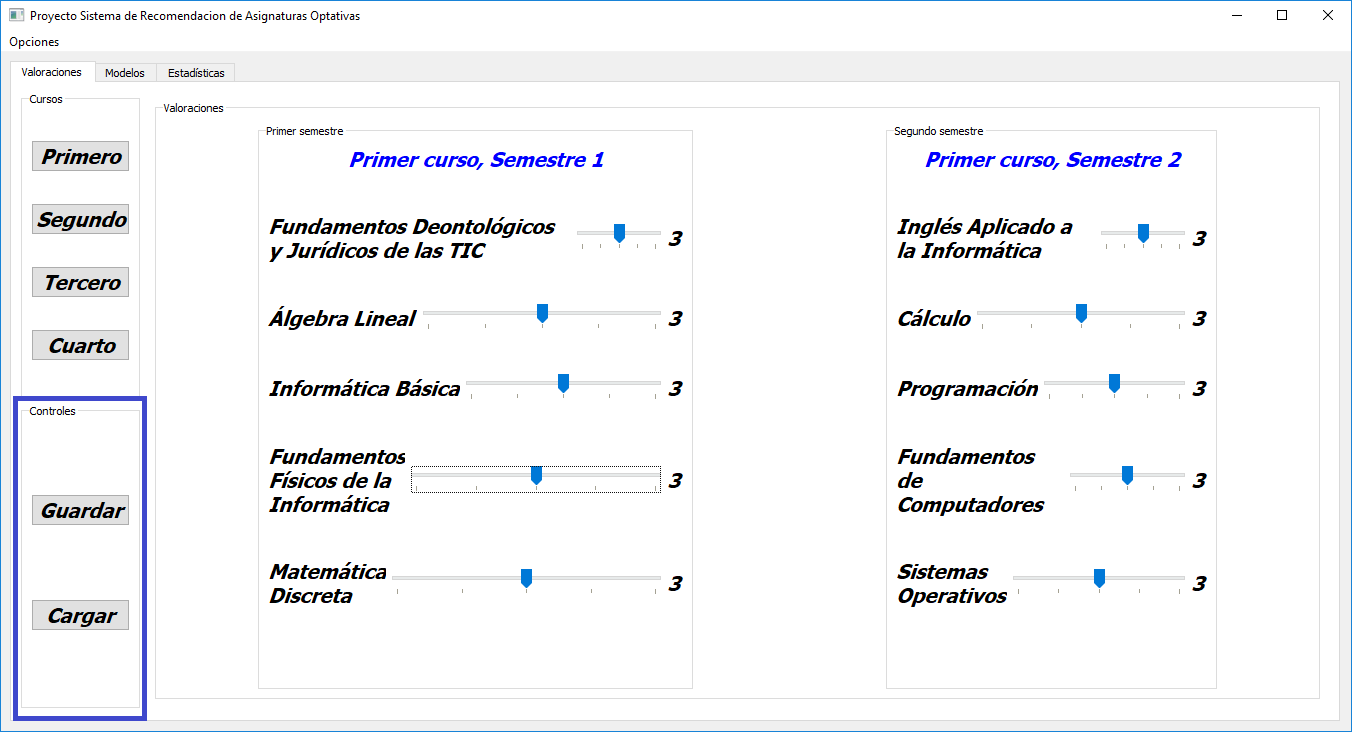
\includegraphics[width=0.80\textwidth]{INTERFAZ_Guarda_Carga}
\caption{Carga y guardado de datos}
\label{fig:E.2.5}
\end{figure}


\subsubsection{Version1.1}
La versión que será entregada de forma definitiva, y que será entregada al tribunal varía levemente en la interfaz gráfica. Al igual que en la Versión 1.0, aparece dicha ventana tras iniciar sesión. La ventana para la ponderación de las asignaturas tiene el siguiente aspecto: \ref{fig:E.2.5.1}
\begin{figure}[h]
\centering
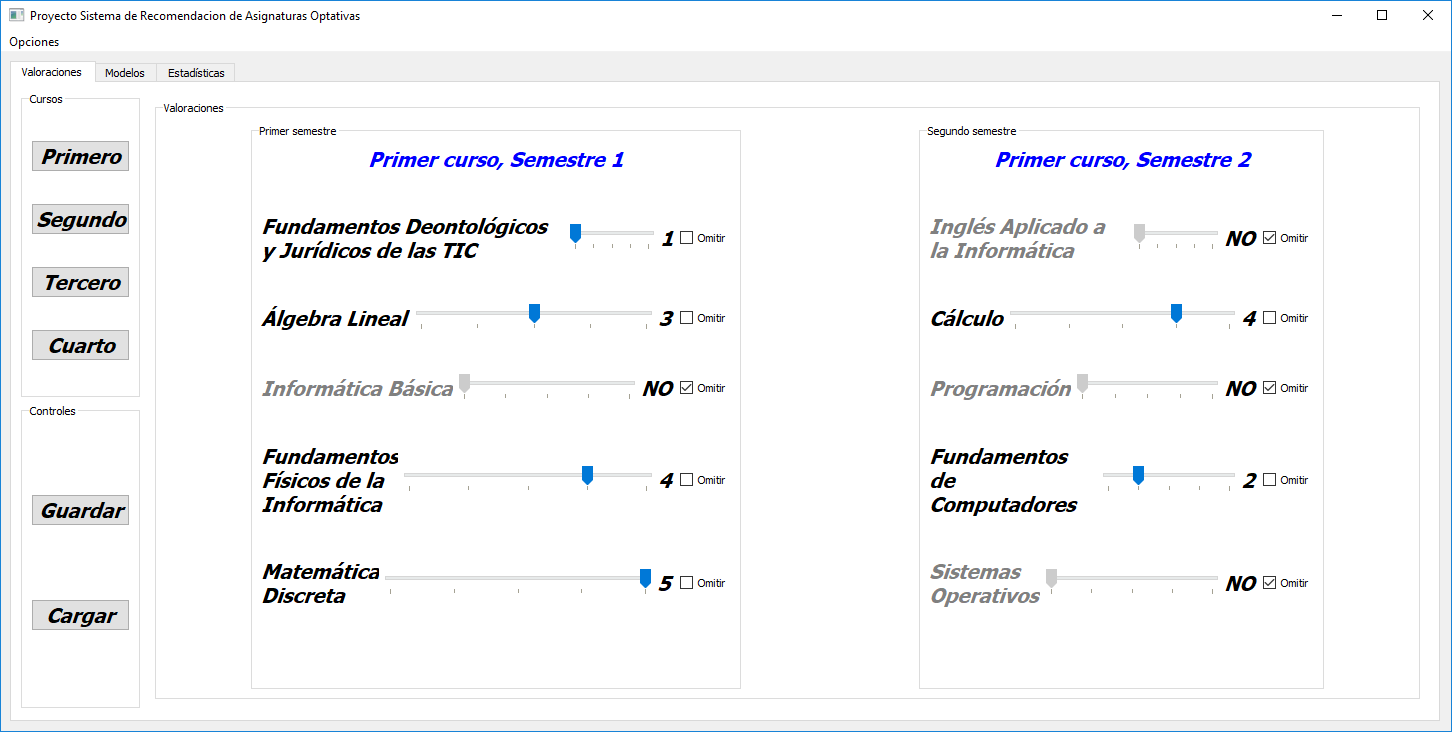
\includegraphics[width=0.80\textwidth]{INTERFAZ_1_1_Principal}
\caption{Pestaña principal versión 1.1}
\label{fig:E.2.5.1}
\end{figure}
\\Ahí radica la diferencia, en la posibilidad de no aplicar una asignatura determinada. Este cambio se debe a que hay alumnos que han convalidado ciertas asignaturas y no las han cursado en el Grado de Ingeniería Informática.\ref{fig:E.2.5.2}
\begin{figure}[h]
\centering
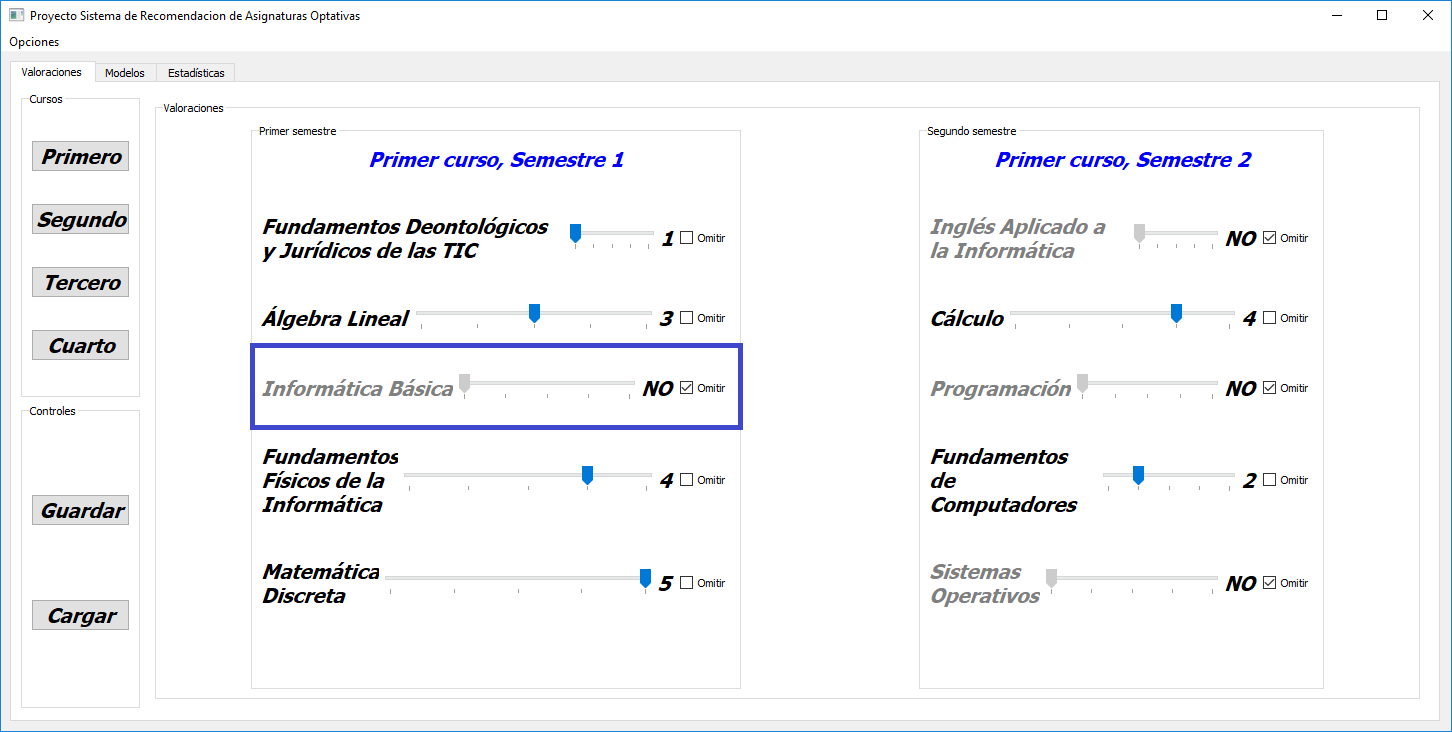
\includegraphics[width=0.80\textwidth]{INTERFAZ_1_1_Diferencia}
\caption{Diferencia respecto a la  versión 1.0}
\label{fig:E.2.5.2}
\end{figure} 
Exceptuando dicho cambio, el resto de las funcionalidades permanecen invariables. 

\subsection{Segunda pestaña}
La segunda pestaña, con las recomendaciones obtenidas, tienen el siguiente aspecto \ref{fig:E.2.6}
\begin{figure}[h]
\centering
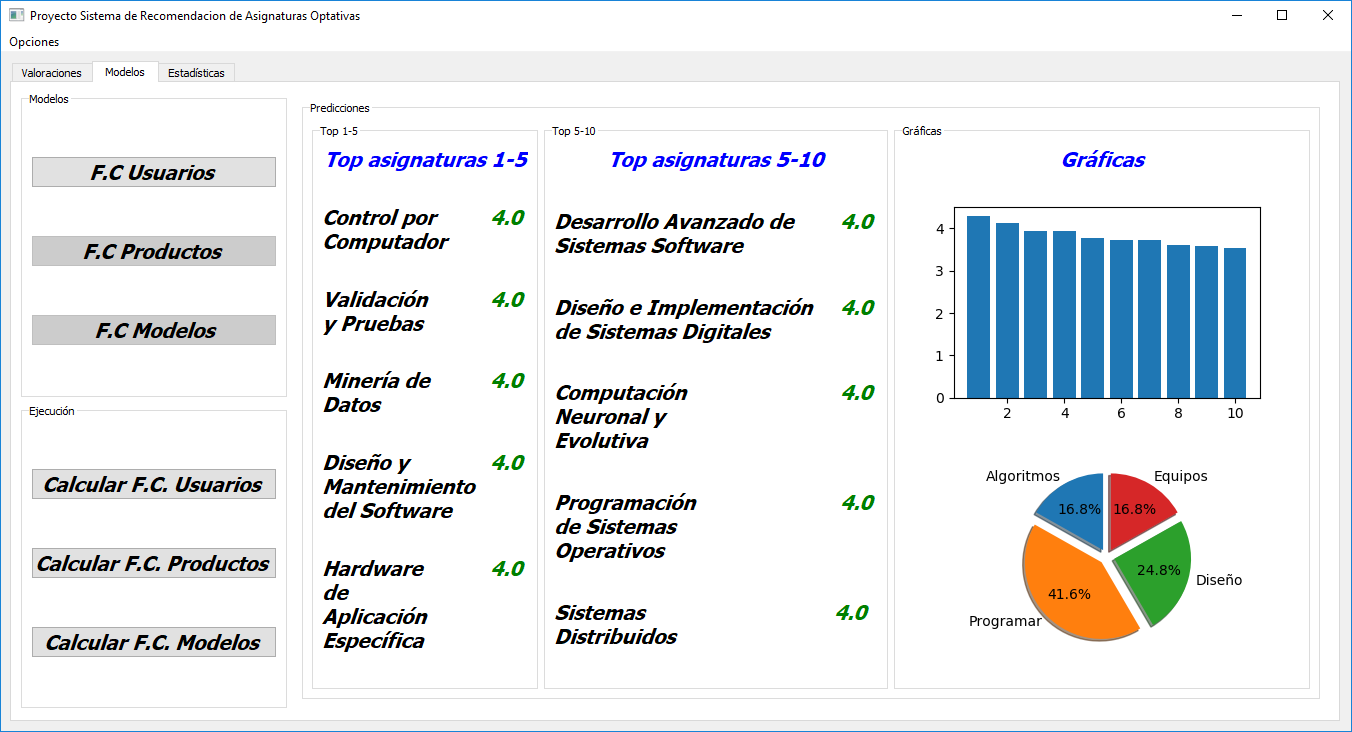
\includegraphics[width=0.80\textwidth]{INTERFAZ_Recomendacion_V1-0}
\caption{Recomendación por defecto}
\label{fig:E.2.6}
\end{figure}
La funcionalidad de dicha pestaña se puede subdividir en: 
\subsubsection{Selección y carga del sistema de recomendación}
El área izquierda se utiliza para seleccionar el sistema de recomendación, siendo por defecto el F.C basado en memoria basado en Usuarios, estando deshabilitados los demás filtros colaborativos. \ref{fig:E.2.7} \\Como se puede observar, únicamente el primer filtro se encuentra habilitado, mientras que los dos sucesivos (basado en productos y  Filtro Colaborativo basado en modelo) se encuentran deshabilitados. 
\begin{figure}[h]
\centering
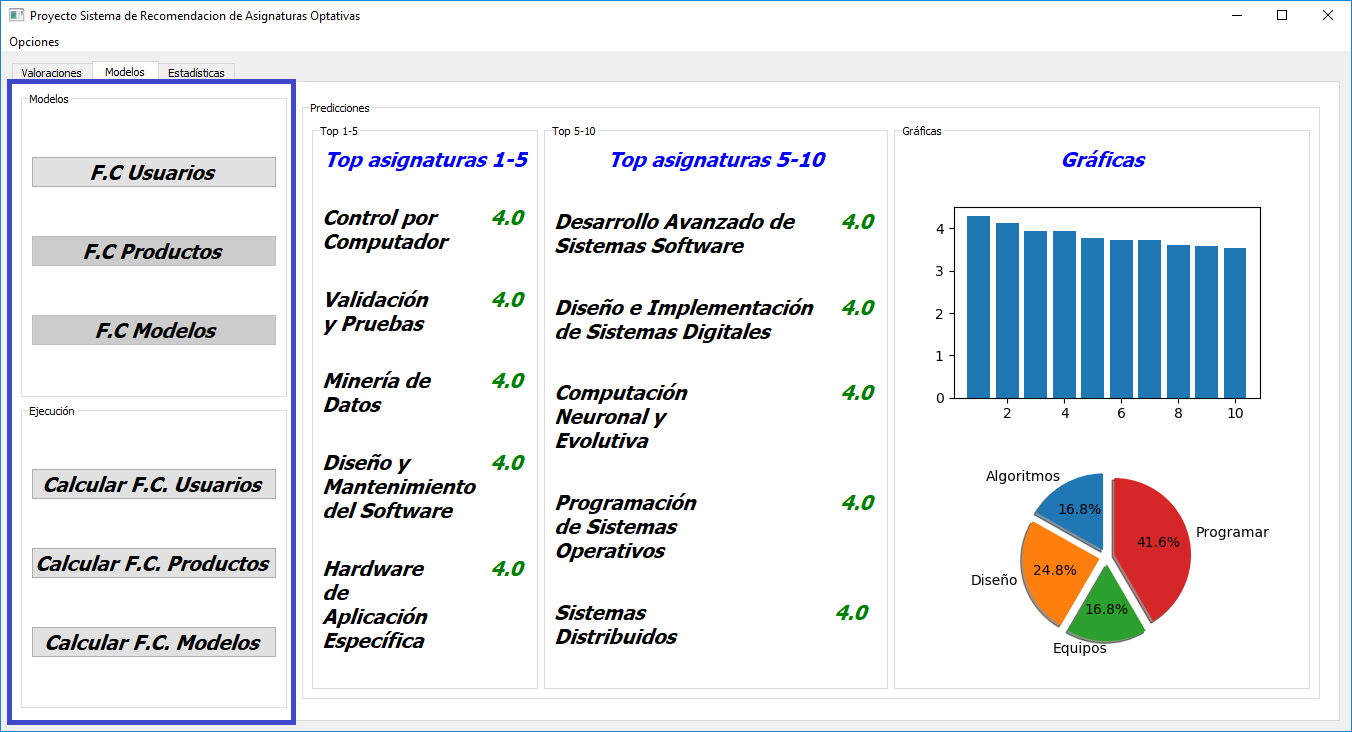
\includegraphics[width=0.80\textwidth]{INTERFAZ_seleccion_V1-0}
\caption{Muestra de los botones deshabilitados}
\label{fig:E.2.7}
\end{figure}
En cambio, si pulsamos el botón "Cargar F.C Productos" se habilita automáticamente la muestra de datos del Filtro Colaborativo basado en Productos. Esto lo podemos observar en la siguiente imagen, \ref{fig:E.2.8} en donde se ha pulsado el botón para el ejemplo. 
\begin{figure}[h]
\centering
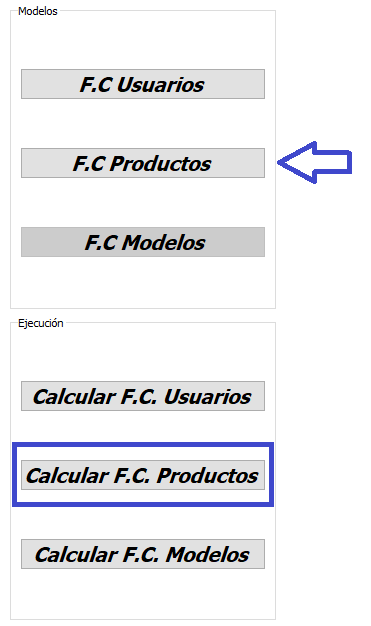
\includegraphics[width=0.80\textwidth]{INTERFAZ_seleccion2_V1-0}
\caption{Muestra de los botones habilitados tras pulsar cargar}
\label{fig:E.2.8}
\end{figure}
\\
Por otro lado, el área central indica las calificaciones redondeadas de las asignaturas recomendadas, con valores del 1-5, ordenadas de forma descendente.\ref{fig:E.2.9} 
\begin{figure}[h]
\centering
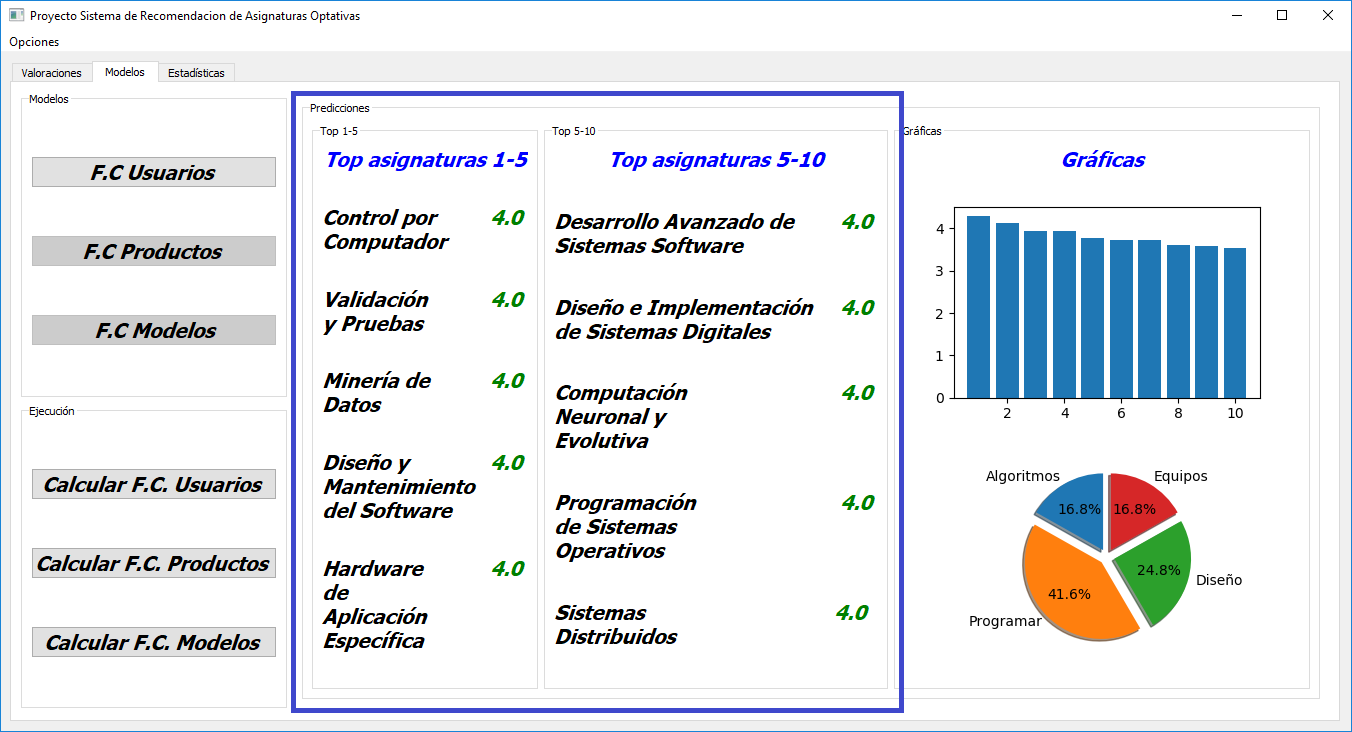
\includegraphics[width=0.80\textwidth]{INTERFAZ_Recomendacion_Asignaturas_V1-0}
\caption{Muestra de los resultados de un filtro colaborativo}
\label{fig:E.2.9}
\end{figure}
Para poder observar los valores reales que nos ha ofrecido el sistema de recomendación, deberíamos observar la gráfica de la derecha, en donde las calificaciones no están redondeadas. Para diferenciarlas, basta con colocar el ratón sobre una asignatura para observar el número de la asignatura, y poder verlo en la gráfica. \ref{fig:E.2.10} 
\begin{figure}[h]
\centering
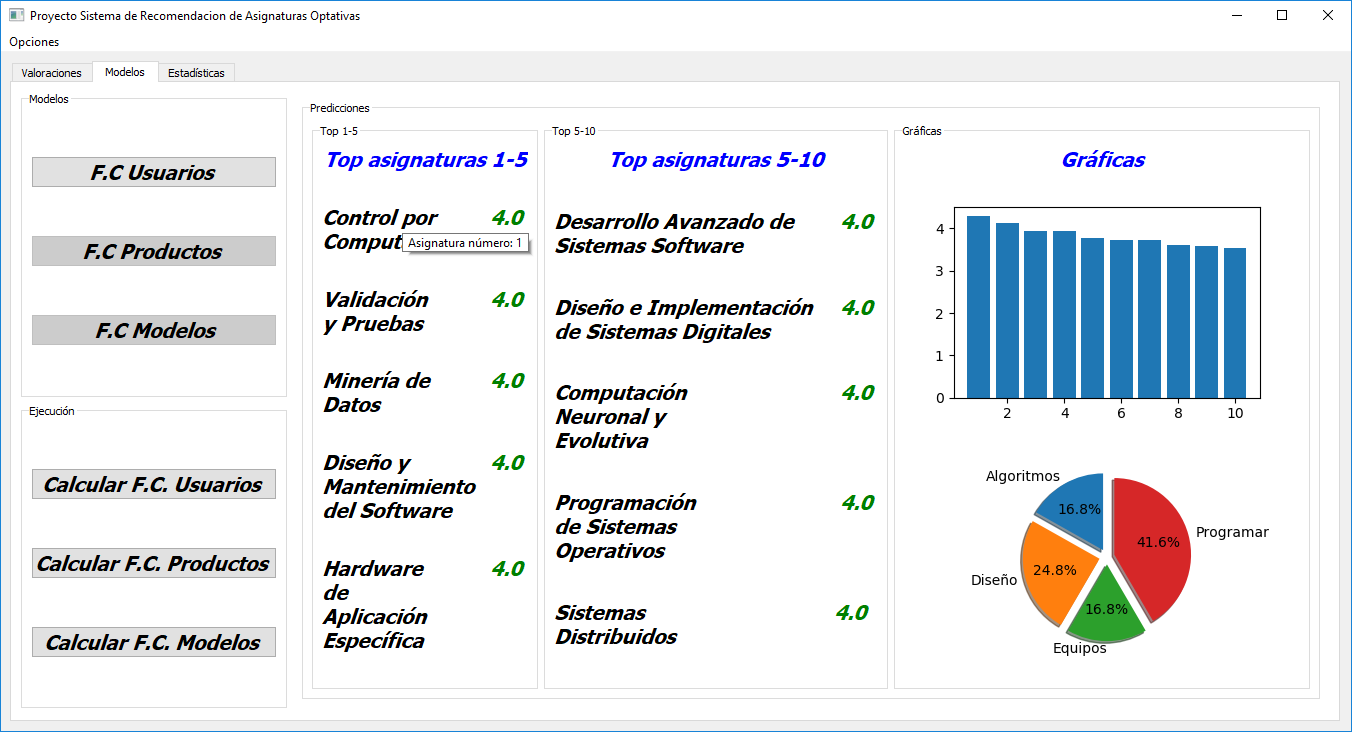
\includegraphics[width=0.80\textwidth]{INTERFAZ_Rellenado_Valores_V1-0}
\caption{Muestra del orden de la asignatura en la gráfica}
\label{fig:E.2.10}
\end{figure}
Así, podemos ver que, "Control por Computador", es la asignatura 1, por lo que en la gráfica, será la primera barra, con una ponderación ligeramente superior al 4. De esta forma, se puede observar que no todas las asignaturas tienen una calificación de 4, por lo que la gráfica de barras resulta útil para ver las diferencias entre las asignaturas. \ref{fig:E.2.11} 
\begin{figure}[h]
\centering
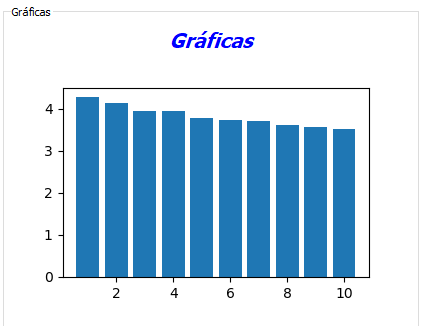
\includegraphics[width=0.80\textwidth]{INTERFAZ_Grafica_V1-0}
\caption{Muestra de la gráfica de asignaturas recomendadas}
\label{fig:E.2.11}
\end{figure}
\\Por otra parte, también tenemos un gráfico que indica las preferencias en los diferentes áreas del usuario, para indicar qué campos son de mayor interés para el mismo, de forma que el usuario pueda conocer el campo por el que se podría decantar en un futuro. \ref{fig:E.2.12} 
\begin{figure}[h]
\centering
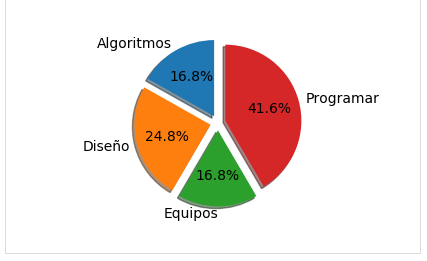
\includegraphics[width=0.80\textwidth]{INTERFAZ_Areas_V1-0}
\caption{Muestra de la gráfica de campos preferentes}
\label{fig:E.2.12}
\end{figure}
\\
Se debe tener en cuenta que dos sistemas de recomendación pueden ofrecer dos resultados diferentes para una misma asignatura, por lo que dichos resultados son meramente informativos. 

\subsection{Tercera pestaña}
La tercera pestaña contiene las medias, medianas, máximos y mínimos de las calificaciones insertadas por los usuarios de forma previa. De esta manera, se puede ver las relaciones de lo que ha seleccionado el usuario y las preferencias del resto de los usuarios. 
\\Las asignaturas se dividen en cursos, de forma que se puede ver las gráficas por cursos, siguiendo el patrón de la primera pestaña. 
\\La estructura de la pestaña tiene el siguiente aspecto: \ref{fig:E.2.13} 
\begin{figure}[h]
\centering
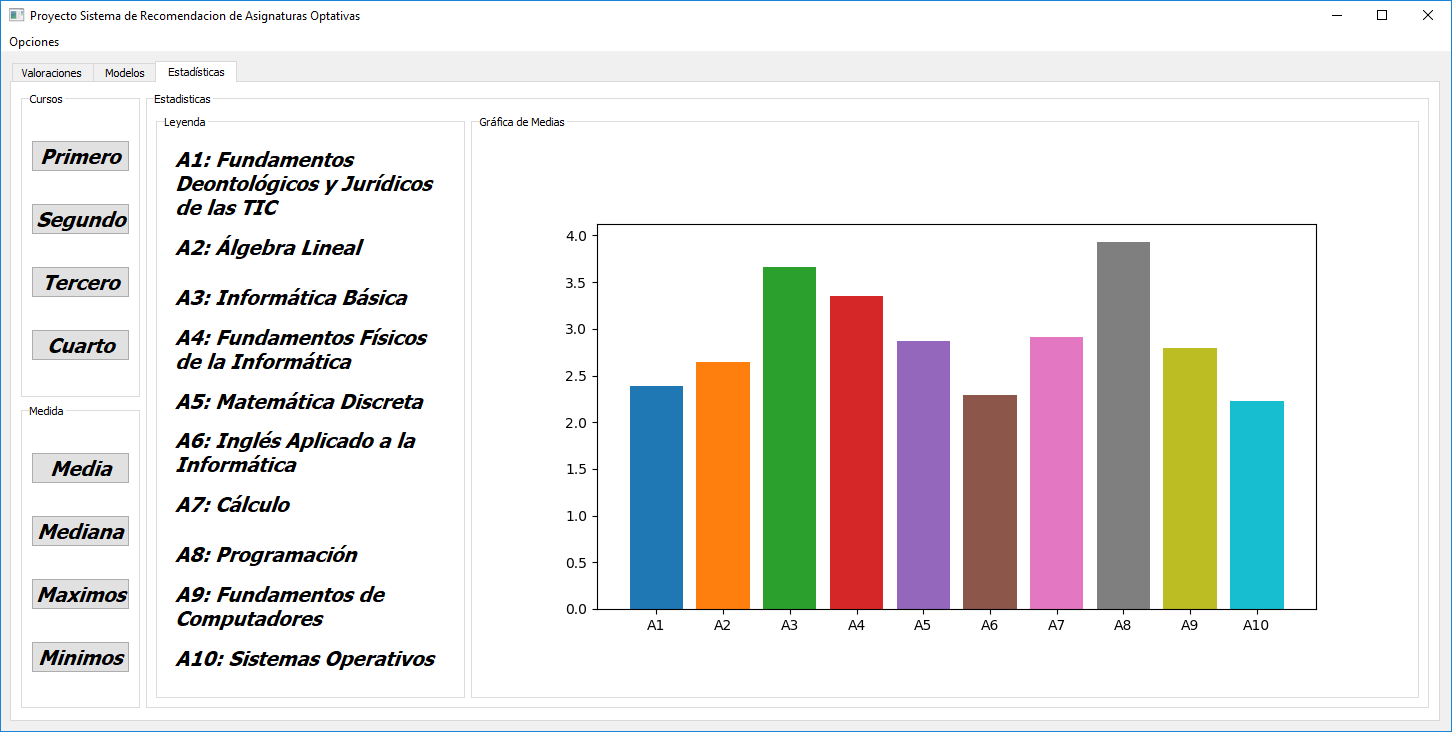
\includegraphics[width=0.80\textwidth]{INTERFAZ_Estadistica}
\caption{Muestra de la pestaña de estadísticas}
\label{fig:E.2.13}
\end{figure}
\\\\Al pulsar los diferentes cursos, obtenemos las pestañas, en donde en la leyenda indica el nombre de la asignatura y en la gráfica de barras su resultado. \ref{fig:E.2.14} 
\begin{figure}[h]
\centering
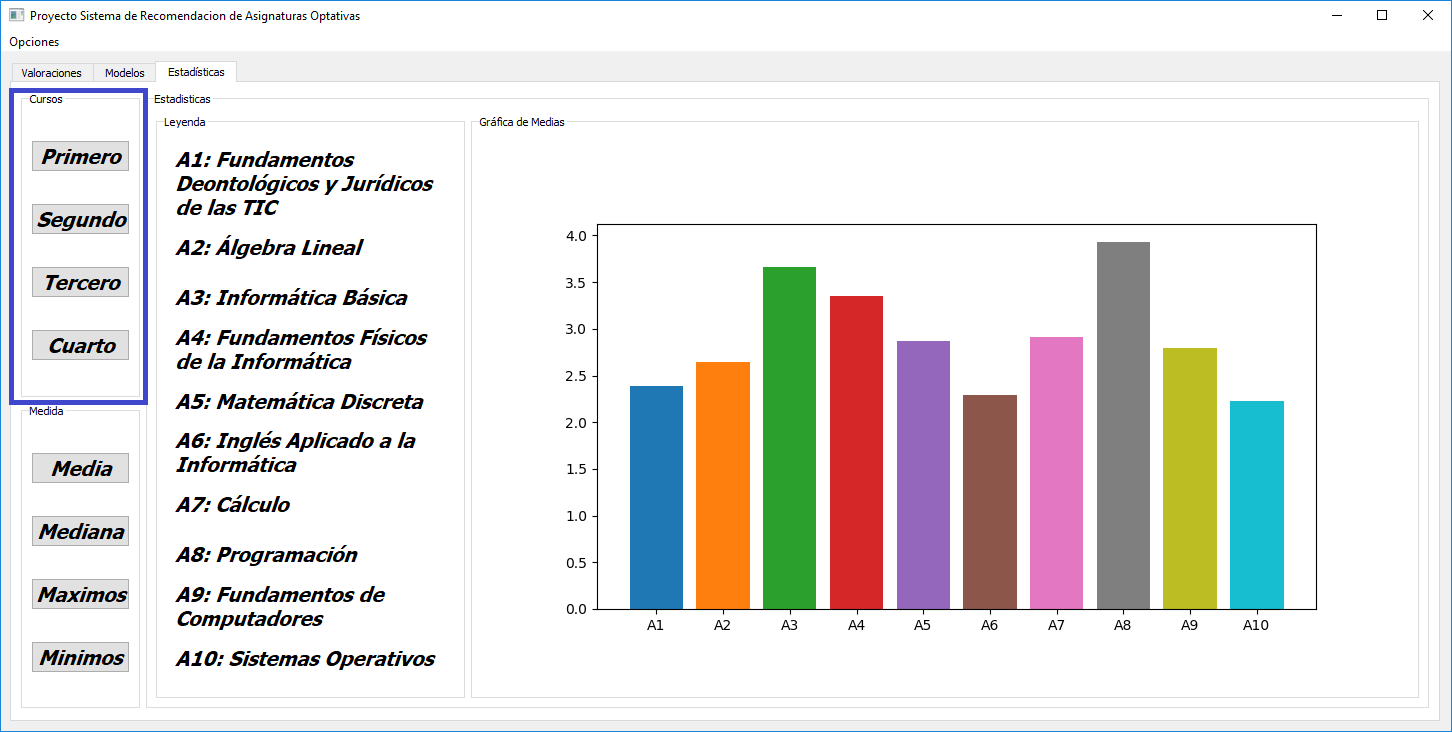
\includegraphics[width=0.80\textwidth]{INTERFAZ_Estadistica_cursos}
\caption{Muestra de los botones de la pestaña}
\label{fig:E.2.14}
\end{figure}
\\Tras seleccionar un curso deseado, automáticamente se calculan los valores de la modalidad en la que se esté (Medias, Medianas, Máximos y Mínimos), cambiándose automáticamente tanto la leyenda de las asignaturas como las ponderaciones. \ref{fig:E.2.15} 
\begin{figure}[h]
\centering
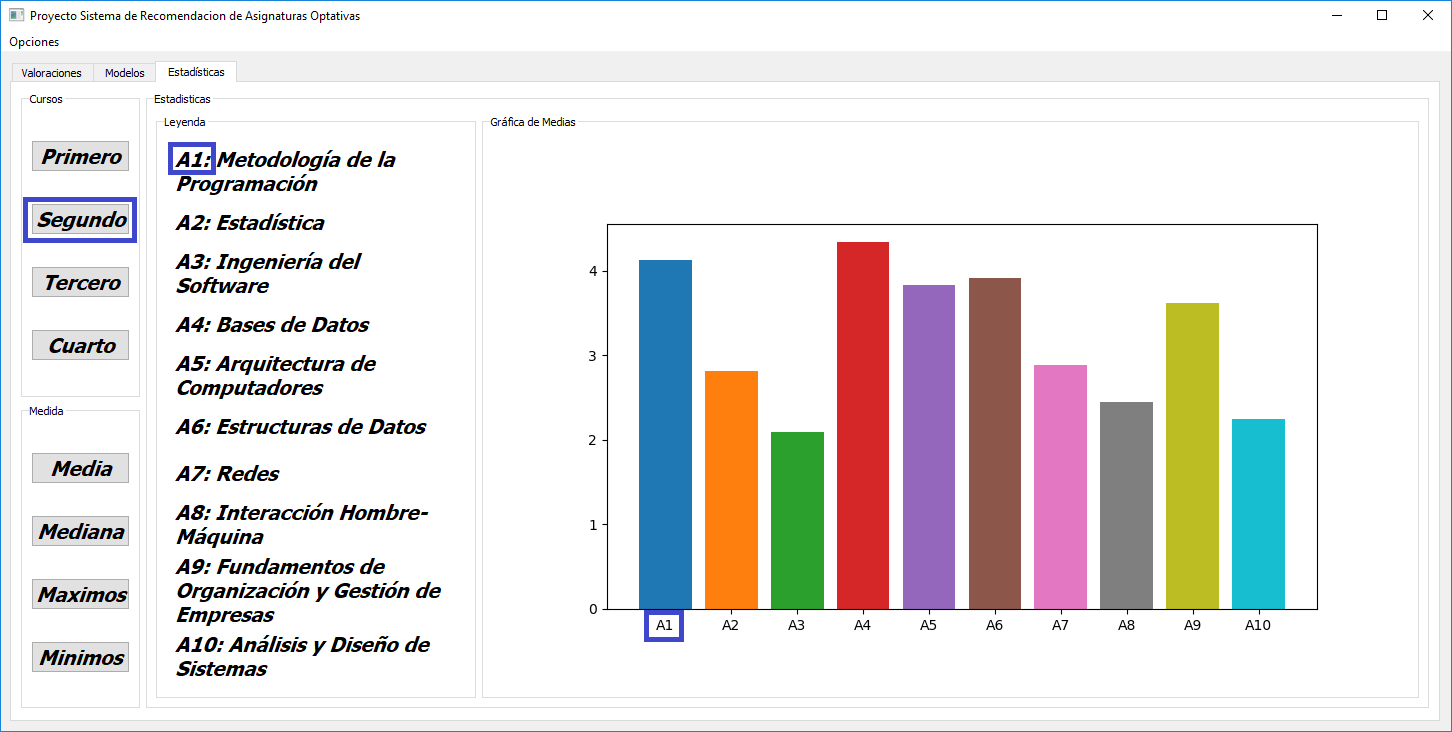
\includegraphics[width=0.80\textwidth]{INTERFAZ_Estadistica_media}
\caption{Ejemplo de media del segundo curso}
\label{fig:E.2.15}
\end{figure}
\\ De esta forma, podemos observar, que en el segundo curso, la asignatura A1 (Metodología de la Programación) tiene una media global de votaciones superior al cuatro. 
\\ Los máximos y mínimos corresponden con la calificación máxima y la mínima de las asignaturas entre los usuarios, de forma que, por ejemplo, para el cuarto curso, la calificación máxima de Diseño e Implementación de Sistemas Digitales es un 5 \ref{fig:E.2.16}, 
\begin{figure}[h]
\centering
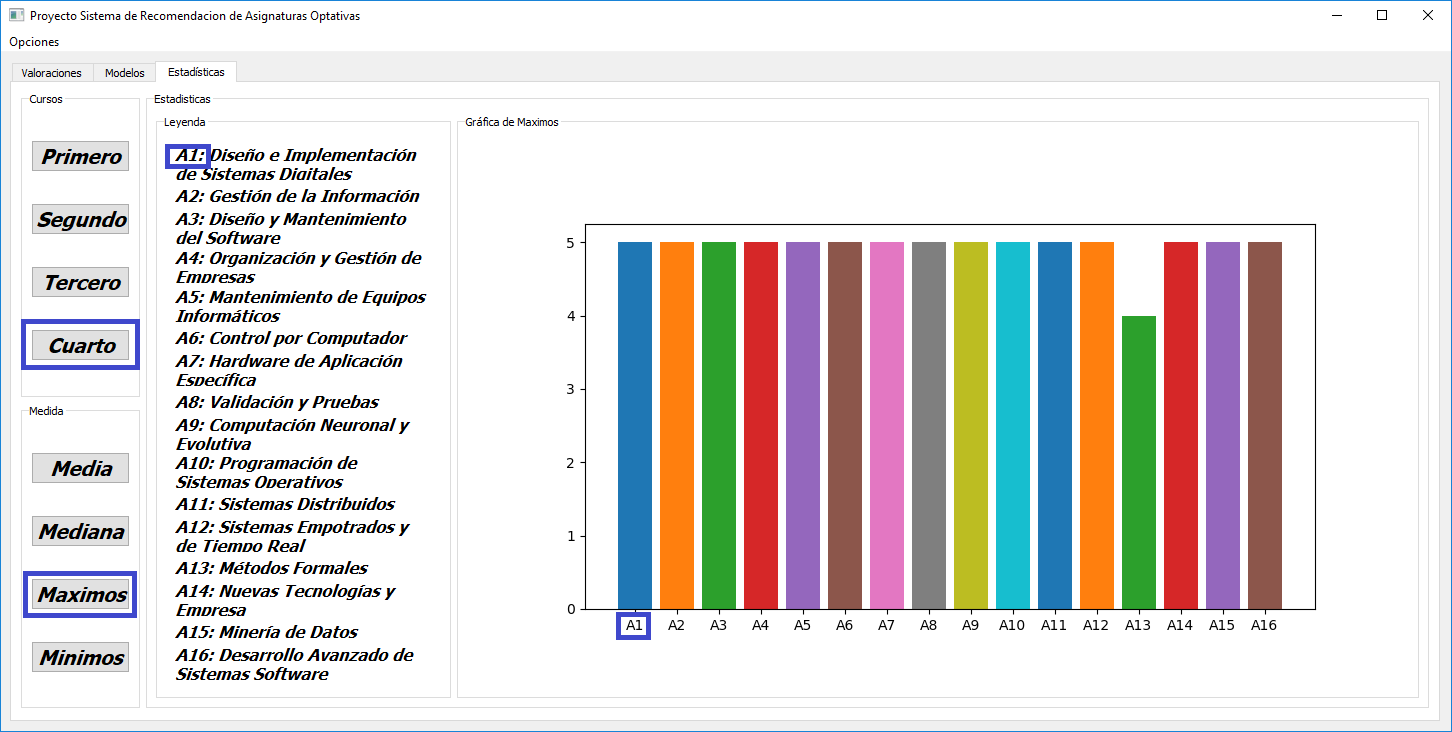
\includegraphics[width=0.80\textwidth]{INTERFAZ_Estadistica_maximos}
\caption{Ejemplo de máximos del cuarto curso}
\label{fig:E.2.16}
\end{figure}
mientras que el mínimo es un 1. \ref{fig:E.2.17}, 
\begin{figure}[h]
\centering
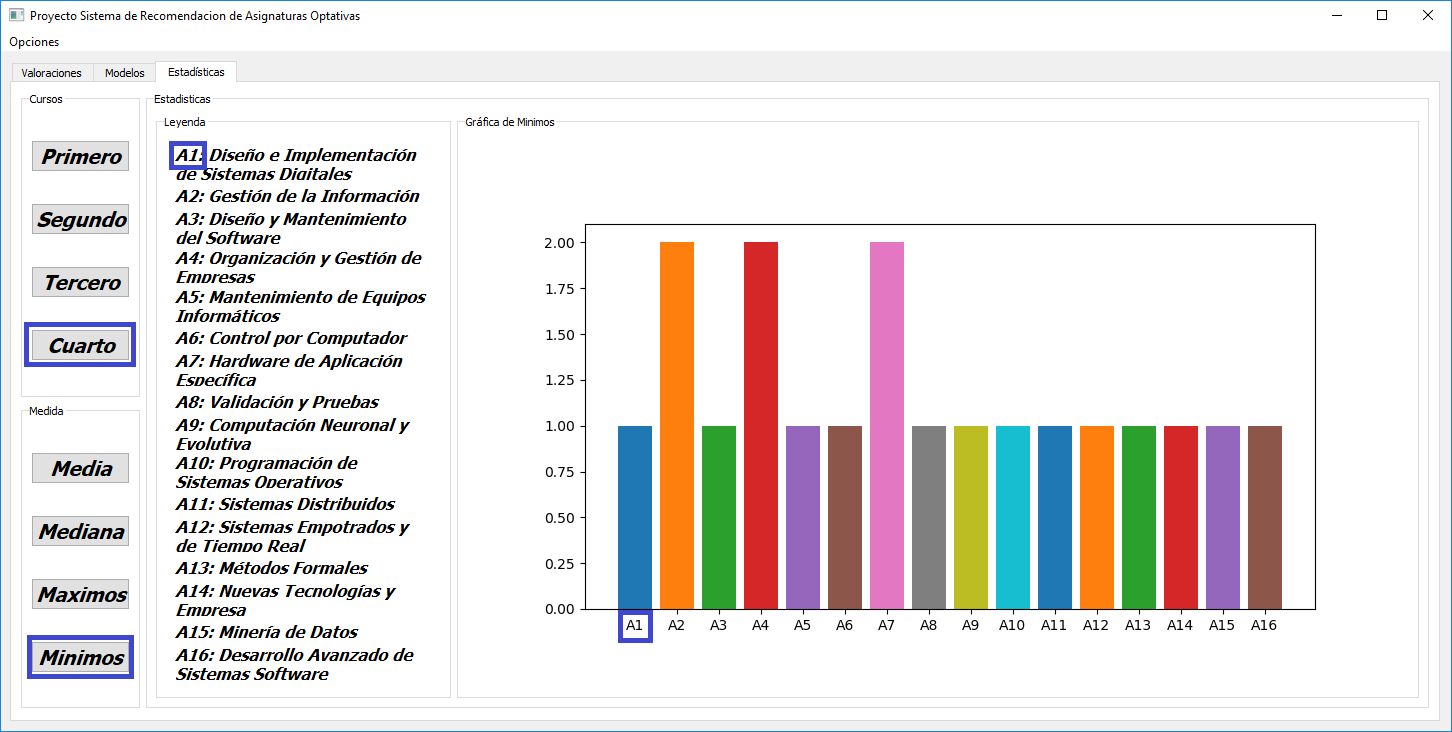
\includegraphics[width=0.80\textwidth]{INTERFAZ_Estadistica_minimos}
\caption{Ejemplo de mínimos del cuarto curso}
\label{fig:E.2.17}
\end{figure}






